\chapter{Numerical Results} \label{chap:results}

In this chapter we demonstrate some results from applying our approach to pairs of steady-state models, implemented using the \texttt{libMesh} library \cite{libMeshPaper}. In Section \ref{sec:cdvcdr}, we demonstrate the results using two models that differ in the physics modeled. In Section \ref{sec:constvfield}, the two models differ in the space to which the parameter belongs. In Section \ref{sec:costAnaly} we discuss the numerical costs of our approach.

%------------------------------------------------------------------------------%
\section{Convection-Diffusion and Convection-Diffusion-Reaction Models}  \label{sec:cdvcdr}
%------------------------------------------------------------------------------%

In this section, we demonstrate the method derived in Section \ref{sec:deriv} for two models which differ in the physics included. We first describe the problem setup, and then present results from applying our approach.

%------------------------------------------------------------%
\subsection{Problem Setup} \label{sec:cdvcdrSetup}
%------------------------------------------------------------%

The high- and low-fidelity models are restricted to a rectangular domain $\Omega$, defined as $\Omega(x_1,x_2)=[0,5]\times[0,1]$, where $x_1$ and $x_2$ are the spatial coordinates. The high-fidelity model is a single-species convection-diffusion-reaction equation with a nonlinear reaction term, described by
\begin{equation}
k_d\nabla^2 u - \vec{V}\cdot\nabla u + k_ru^2= f(q),
\label{eq:cdvcdrHF}
\end{equation}
where the state $u$ is the species concentration, $f(q)$ is a forcing field described by the parameters, $k_d = 0.1$ is a diffusion coefficient and $k_r = -42.0$ is a reaction coefficient. The low-fidelity model
\begin{equation}
k_d\nabla^2 u - \vec{V}\cdot\nabla u = f(q)
\end{equation}
differs only in the removal of the reaction term. Both models share a common velocity field, described by $\vec{V}(x_1,x_2) = (2x_2(1-x_2),0)$. To form the mixed-fidelity models, we divide the domain into complementary subdomains, $\Omega_{HF}$ and $\Omega_{LF}$, where the high- and low-fidelity models are solved, respectively. The resulting mixed-fidelity models can be described by 
\begin{equation}
k_d\nabla^2 u - \vec{V}\cdot\nabla u + k^{MF}_ru^2= f(q),
\end{equation}
where $k^{MF}_r$ is a piecewise-constant reaction coefficient
\begin{equation}
k^{MF}_r=
\begin{cases}
-42.0 & \textrm{if }x\in\Omega_{HF} \\
0 & \textrm{if }x\in\Omega_{LF}.
\end{cases}
\end{equation}
Homogeneous Dirichlet boundary conditions are applied on the entire boundary of the domain.

We let the unknown parameters we wish to infer correspond to the forcing field, so that $f(q)=q$. Observations $d=(u(0.35,0.35),u(1.56,0.61),u(3.1,0.5))$ from three points in the domain are artificially generated by running the high-fidelity model on a finer mesh with a piecewise constant source term $f_{true}$
\begin{equation}
f_{true}(x_1,x_2)=
\begin{cases}
1.0 & \textrm{if }(x_1,x_2)\in[0.125,0.375]\times[0.125,0.375] \\
0.8 & \textrm{if }(x_1,x_2)\in[2.375,2.625]\times[0.375,0.625] \\
0 & \textrm{otherwise}.
\end{cases}
\end{equation}
The QoI we wish to calculate is the integral of the state,
\begin{equation}
I(q,u)=\int_{(x_1,x_2)\in \Omega_I} u \:\textrm{d}A,
\end{equation}
over a region $\Omega_I=[0.625,0.875]\times[0.375,0.625]$. The locations of the observations and the region $\Omega_I$ over which the QoI is calculated is shown in Figure \ref{fig:baseSetup}. Since the inverse problem is ill-posed, we use Tikhonov regularization \cite{EngHanNeu00}; the regularization term is $\frac{\beta}{2}\int_\Omega \|\nabla f(q)\|_2^2\:\textrm{d}A$, where $\beta=10^{-5}$ is a regularization coefficient.

\begin{figure}[h]
\centering
\includegraphics[width=0.8\textwidth]{baseSeries/setup_3_3.pdf}
\caption{Locations of the observations and the QoI region.}
\label{fig:baseSetup}
\end{figure}

For the numerical simulations, we use the \texttt{libMesh} library \cite{libMeshPaper}. The domain is discretized by a regular mesh of quadrilaterals, with 50 and 250 elements along the short and long boundaries, respectively, for a total of 12,500 elements. We implement the finite element method (FEM) for a continuous Galerkin formulation using a linear nodal basis, for a total of 76,806 degrees of freedom. The P\'{e}clet number never exceeds 0.1 in any part of the domain, so we do not require stabilization.

%------------------------------------------------------------%
\subsection{Adaptive Model Refinement} \label{sec:cdvcdrBaseRef} 
%------------------------------------------------------------%

Once the QoI error estimate is calculated using Equation (\ref{eq:finErrExp}), the error estimate is then localized to each element to give an element-wise decomposition of the error. Here we calculate the contribution to the estimated error by a particular element $\kappa$ by simply considering all area integrals in the error estimate expression, limited to that element. As described in Algorithm \ref{alg:refSeries}, based on this element-wise decomposition, we increase the proportion of the domain in which the high-fidelity model is used until the estimated absolute relative error in the QoI is less than $1\%$. In this case, once an element is assigned to the high-fidelity portion of the domain $\Omega_{HF}$, it remains assigned as such for all future subsequent mixed-fidelity models. Figure \ref{fig:baseRef} shows the element-wise decomposition of the error estimate, as well as the subdomains where the low- and high-fidelity models are used, for the series of mixed-fidelity models thus generated. The true and estimated absolute relative errors in the QoI for these same mixed-fidelity models are shown in Figure \ref{fig:baseErr}, while the effectivity index for the error estimate, defined by
\begin{equation}
\textrm{effectivity index}=\frac{\textrm{estimated QoI error}}{\textrm{true QoI error}},
\end{equation}
is shown in Figure \ref{fig:baseErrEff}.

It can be seen that in this case, while the error estimates are not exact due to the nonlinear reaction term in the high-fidelity model, the error estimates are fairly accurate. In addition, the QoI that would have been obtained from solving the inverse problem with the high-fidelity model can be replicated to within $1\%$ with a mixed-fidelity model where the high-fidelity model is used in only $15\%$ of the domain.

\begin{figure}[h!]
\centering
  \begin{subfigure}[b]{\textwidth}
  \centering
    \includegraphics[width=0.48\textwidth]{baseSeries/cd_cdr_LF_divvy.pdf}
    \includegraphics[width=0.49\textwidth]{baseSeries/err_breakdown_LF.pdf}
    \vspace{-0.5\baselineskip}
    \caption{MF$_0$ ($0\%$ HF)}
    \vspace{0.8\baselineskip}
  \end{subfigure}
	\begin{subfigure}[b]{\textwidth}
  \centering
    \includegraphics[width=0.48\textwidth]{baseSeries/cd_cdr_MF01_divvy.pdf}
    \includegraphics[width=0.49\textwidth]{baseSeries/err_breakdown_MF01.pdf}
    \vspace{-0.5\baselineskip}
    \caption{MF$_1$ ($5\%$ HF)}
    \vspace{0.8\baselineskip}
  \end{subfigure}
  \begin{subfigure}[b]{\textwidth}
  \centering
    \includegraphics[width=0.48\textwidth]{baseSeries/cd_cdr_MF02_divvy.pdf}
    \includegraphics[width=0.49\textwidth]{baseSeries/err_breakdown_MF02.pdf}
    \vspace{-0.5\baselineskip}
    \caption{MF$_2$ ($10\%$ HF)}
    \vspace{0.8\baselineskip}
  \end{subfigure}
  \begin{subfigure}[b]{\textwidth}
  \centering
    \includegraphics[width=0.48\textwidth]{baseSeries/cd_cdr_MF03_divvy.pdf}
    \includegraphics[width=0.49\textwidth]{baseSeries/err_breakdown_MF03.pdf}
    \vspace{-0.5\baselineskip}
    \caption{MF$_3$ ($15\%$ HF)}
    \vspace{0.8\baselineskip}
  \end{subfigure}
\caption{Element-wise decomposition of error estimate (right) and domain division (left; low-fidelity convection-diffusion model used in red portion, high-fidelity convection-diffusion-reaction model used in blue portion) for mixed-fidelity models.}
\label{fig:baseRef}
\end{figure}

\begin{figure}[h]
\centering
\includegraphics[width=0.8\textwidth]{baseSeries/err_est.pdf}
\caption{True and estimated absolute relative error in QoI, plotted as a function of the percentage area of the domain in which the high-fidelity convection-diffusion-reaction model is used.}
\label{fig:baseErr}
\end{figure}

\begin{figure}[h]
\centering
\includegraphics[width=0.8\textwidth]{baseSeries/err_eff.pdf}
\caption{Effectivity index of QoI error estimate, plotted as a function of the percentage area of the domain in which the high-fidelity convection-diffusion-reaction model is used.}
\label{fig:baseErrEff}
\end{figure}

\subsection{Interaction of Observations and QoI}

The element-wise decomposition of the error estimate (\ref{eq:finErrExp}) suggests the use of the high-fidelity model in areas of the domain where the parameter field is both informed by the observations and informative about the QoI. To see this, we compare the element-wise decomposition of the error estimate for three sizes of the QoI region $\Omega_I$ given the same set of observations, and for three sets of observations given the same QoI region. Again we increase the proportion of the domain in which the high-fidelity model is used until the estimated absolute relative error in the QoI is less than $1\%$. The element-wise decomposition of the error estimates (from the first three iterations) for the three sizes of the QoI region $\Omega_I$ given the same set of observations is shown in Figure \ref{fig:qoiStudy}, and for the three sets of observations given the same QoI region is shown in Figure \ref{fig:dataStudy}. For the three cases where the observations were fixed but the QoI region allowed to vary, more iterations were required as the QoI region expanded; only the first three iterations are shown in Figure \ref{fig:qoiStudy}. For the three cases where the QoI region was fixed but the set of observations allowed to vary, only three iterations were required to achieve an estimated absolute relative QoI error of less than $1\%$; all three iterations are shown in Figure \ref{fig:dataStudy}. 

\begin{figure}
\captionsetup[subfigure]{justification=centering}
\centering
  \begin{subfigure}[t]{0.191\textwidth}
  \centering
    \includegraphics[width=\textwidth]{vs_qoi/setup_5_3.pdf}
    \includegraphics[width=\textwidth]{vs_qoi/setup_7_3.pdf}
    \includegraphics[width=\textwidth]{vs_qoi/setup_3_3.pdf}
    \caption{Locations of observations and QoI region $\Omega_I$}
    \label{subfig:obsSetup}
  \end{subfigure}
  \begin{subfigure}[t]{0.155\textwidth}
  \centering
    \includegraphics[width=\textwidth]{vs_qoi/qoi5_sens3/err_breakdown_LF.pdf}
    \includegraphics[width=\textwidth]{vs_qoi/qoi7_sens3/err_breakdown_LF.pdf}
    \includegraphics[width=\textwidth]{vs_qoi/qoi3_sens3/err_breakdown_LF.pdf}
    \caption{MF$_0$ \\ ($0\%$ HF)}
    \label{subfig:obsLF}
  \end{subfigure}
  \begin{subfigure}[t]{0.155\textwidth}
  \centering
    \includegraphics[width=\textwidth]{vs_qoi/qoi5_sens3/err_breakdown_MF01.pdf}
    \includegraphics[width=\textwidth]{vs_qoi/qoi7_sens3/err_breakdown_MF01.pdf}
    \includegraphics[width=\textwidth]{vs_qoi/qoi3_sens3/err_breakdown_MF01.pdf}
    \caption{MF$_1$ \\ ($5\%$ HF)}
  \end{subfigure}
  \begin{subfigure}[t]{0.155\textwidth}
  \centering
    \includegraphics[width=\textwidth]{vs_qoi/qoi5_sens3/err_breakdown_MF02.pdf}
    \includegraphics[width=\textwidth]{vs_qoi/qoi7_sens3/err_breakdown_MF02.pdf}
    \includegraphics[width=\textwidth]{vs_qoi/qoi3_sens3/err_breakdown_MF02.pdf}
    \caption{MF$_2$ \\ ($10\%$ HF)}
  \end{subfigure}
  \begin{subfigure}[t]{0.243\textwidth}
  \centering
    \includegraphics[width=\textwidth]{vs_qoi/qoi5_sens3/err_breakdown_MF03.pdf}
    \includegraphics[width=\textwidth]{vs_qoi/qoi7_sens3/err_breakdown_MF03.pdf}
    \includegraphics[width=\textwidth]{vs_qoi/qoi3_sens3/err_breakdown_MF03.pdf}
    \caption{MF$_3$ \\ ($15\%$ HF)}
    \label{subfig:obsMFlast}
  \end{subfigure}
  \caption{Compare the element-wise decomposition of the error estimates (\subref{subfig:obsLF}-\subref{subfig:obsMFlast}), given the same observations (teal points in (\subref{subfig:obsSetup})) and varying QoI region (purple box in (\subref{subfig:obsSetup})).}
  \label{fig:qoiStudy}
\end{figure}

\begin{figure}
\captionsetup[subfigure]{justification=centering}
\centering
  \begin{subfigure}[t]{0.191\textwidth}
  \centering
    \includegraphics[width=\textwidth]{vs_data/setup_3_10.pdf}
    \includegraphics[width=\textwidth]{vs_data/setup_3_5.pdf}
    \includegraphics[width=\textwidth]{vs_data/setup_3_3.pdf}
    \caption{Locations of observations and QoI region $\Omega_I$}
    \label{subfig:obsSetup}
  \end{subfigure}
  \begin{subfigure}[t]{0.155\textwidth}
  \centering
    \includegraphics[width=\textwidth]{vs_data/qoi3_sens10/err_breakdown_LF.pdf}
    \includegraphics[width=\textwidth]{vs_data/qoi3_sens5/err_breakdown_LF.pdf}
    \includegraphics[width=\textwidth]{vs_data/qoi3_sens3/err_breakdown_LF.pdf}
    \caption{MF$_0$ \\ ($0\%$ HF)}
    \label{subfig:obsLF}
  \end{subfigure}
  \begin{subfigure}[t]{0.155\textwidth}
  \centering
    \includegraphics[width=\textwidth]{vs_data/qoi3_sens10/err_breakdown_MF01.pdf}
    \includegraphics[width=\textwidth]{vs_data/qoi3_sens5/err_breakdown_MF01.pdf}
    \includegraphics[width=\textwidth]{vs_data/qoi3_sens3/err_breakdown_MF01.pdf}
    \caption{MF$_1$ \\ ($5\%$ HF)}
  \end{subfigure}
  \begin{subfigure}[t]{0.155\textwidth}
  \centering
    \includegraphics[width=\textwidth]{vs_data/qoi3_sens10/err_breakdown_MF02.pdf}
    \includegraphics[width=\textwidth]{vs_data/qoi3_sens5/err_breakdown_MF02.pdf}
    \includegraphics[width=\textwidth]{vs_data/qoi3_sens3/err_breakdown_MF02.pdf}
    \caption{MF$_2$ \\ ($10\%$ HF)}
  \end{subfigure}
  \begin{subfigure}[t]{0.245\textwidth}
  \centering
    \includegraphics[width=\textwidth]{vs_data/qoi3_sens10/err_breakdown_MF03.pdf}
    \includegraphics[width=\textwidth]{vs_data/qoi3_sens5/err_breakdown_MF03.pdf}
    \includegraphics[width=\textwidth]{vs_data/qoi3_sens3/err_breakdown_MF03.pdf}
    \caption{MF$_3$ \\ ($15\%$ HF)}
    \label{subfig:obsMFlast}
  \end{subfigure}
  \caption{Compare the element-wise decomposition of the error estimates (\subref{subfig:obsLF}-\subref{subfig:obsMFlast}), given the same QoI region (purple box in (\subref{subfig:obsSetup})) and varying observations (teal points in (\subref{subfig:obsSetup})).}
  \label{fig:dataStudy}
\end{figure}

The convective aspect of the models causes information to flow with the velocity field, and the diffusive aspect causes information to spread locally. Thus, it is expected that it would be most important to use the high-fidelity model in the QoI region, and in areas around observations upstream and just downstream of the QoI region. Using the high-fidelity model around observations is expected to become less important as the observations are placed further downstream from the QoI region. These expectations are supported by the results. For this pair of models and a QoI that is the integral of the state over a region, an appropriate mixed-fidelity model could have been designed by intuition. However, the interaction between the observations and the QoI may not always be so intuitive, and it is in these cases that a rigorous method for forming a mixed-fidelity model would be most helpful.

%\subsection{Effect of Regularization} %removed; more regularization doesn't seem to imply you can stop refining sooner...

\subsection{Highly Nonlinear Problems} \label{sec:solveRob}

For a highly nonlinear high-fidelity model, it may sometimes be the case that solving the inverse problem requires a more complex or specialized optimization algorithm; for example, one may need to use continuation methods (such as in \cite{BaoLiu03}), or utilize a problem-specific preconditioner (such as in \cite{Hanke00}). However, solving the inverse problem with a mixed-fidelity model, where this high-fidelity model is only used in a small portion of the domain, may be achievable using a simpler optimization algorithm. In this subsection, we give an example of such a case.

To solve the inverse problem, we use the default nonlinear solver in \texttt{libMesh} (Newton's method with Brent line-search) to solve the optimality conditions of the corresponding optimization problem (see Equation \ref{eq:invOpt}). Keeping most of the setup described in Section \ref{sec:cdvcdrSetup}, we consider a different high-fidelity model, one where the magnitude of the reaction coefficient in Equation (\ref{eq:cdvcdrHF}) is increased from $k_r=-42$ to $k_r=-442$; let this new model be denoted by HF$_{442}$. We can no longer simply use the default nonlinear solver in \texttt{libMesh} to solve the inverse problem with this new, more nonlinear high-fidelity model, as the solver fails to converge. Convergence can be achieved by using continuation; we solve the inverse problem for a sequence of models, varying the reaction coefficient in Equation (\ref{eq:cdvcdrHF}) from $k_r=-42$ to $k_r=-442$ at intervals of 50, and using the solution of one problem as the initial guess for the next.

Alternatively, we use Algorithm \ref{alg:refSeries} to generate a series of mixed-fidelity models using the low-fidelity model and the HF$_{442}$ model. The inverse problem can be solved for these mixed-fidelity models using the default nonlinear solver, and we are able to achieve an estimated relative QoI error of less than $1\%$ with a mixed-fidelity model where the high-fidelity model is used in only $25\%$ of the domain, as shown in Figure~\ref{fig:442Err}. Figure \ref{fig:442ErrEff} gives the effectivity index of the error estimates.

\begin{figure}[h]
\centering
\includegraphics[width=0.8\textwidth]{442/err_est.pdf}
\caption{Estimated absolute relative error in QoI, plotted as a function of the percentage area of the domain in which the high-fidelity convection-diffusion-reaction model, with $k_r=-442$, is used.}
\label{fig:442Err}
\end{figure}

\begin{figure}[h]
\centering
\includegraphics[width=0.8\textwidth]{442/err_eff.pdf}
\caption{Effectivity index of QoI error estimate, plotted as a function of the percentage area of the domain in which the high-fidelity convection-diffusion-reaction model, with $k_r=-442$, is used.}
\label{fig:442ErrEff}
\end{figure}

%------------------------------------------------------------------------------%
\section{Constant versus Field Parameters}  \label{sec:constvfield}
%------------------------------------------------------------------------------%

In this section, we consider two models which differ in the space to which the parameter belongs. We first describe the problem setup, and then present results from applying our approach.

%------------------------------------------------------------%
\subsection{Problem Setup} %\label{sec:svfSetup}
%------------------------------------------------------------%

The high-fidelity model 
\begin{equation}
k_d\nabla^2 u - \vec{V}\cdot\nabla u + k_ru^2= f(q),\quad q\in U,
\end{equation}
is again a single-species convection-diffusion-reaction equation with a nonlinear reaction term, where $k_d = 0.1$ is a diffusion coefficient and $k_r = -4.2$ is a reaction coefficient. The low-fidelity model
\begin{equation}
k_d\nabla^2 u - \vec{V}\cdot\nabla u + k_ru^2= f(q),\quad q\in\R
\end{equation}
differs from the high-fidelity model only in that the parameter $q$ is a constant instead of a field. Then the intermediate mixed-fidelity models have parameter fields which are non-constant in only portions of the domain. For ease of implementation, we require that the resulting parameter field remain continuous at the interface between the low-fidelity and high-fidelity subdomains, although this constraint is not necessary for the theory to hold. The velocity field and boundary conditions, as well as the observations, unknown parameters to be inferred, and QoI, remain the same as described in Section~\ref{sec:cdvcdr}. As the inverse problem is ill-posed, except for perhaps in the case where the low-fidelity model is used throughout the domain, regularization is added; the Tikhonov regularization term is $\frac{\beta}{2}\int_\Omega \|\nabla f(q)\|_2^2+f(q)^2\:\textrm{d}A$, where $\beta=10^{-3}$ is a regularization coefficient. For this case, the domain is discretized by a regular mesh of quadrilaterals, with 15 and 75 elements along the short and long boundaries, respectively, for a total of 11,250 elements. The P\'{e}clet number never exceeds 0.34 in any part of the domain, so we do not require stabilization.

%------------------------------------------------------------%
\subsection{Adaptive Model Refinement} %\label{sec:svfBaseRef}
%------------------------------------------------------------%

Based on the element-wise decomposition of the estimated error, we increase the proportion of the domain in which the high-fidelity field representation model is used until the estimated absolute relative error in the QoI is less than $5\%$. In this case, we allow an element assigned to $\Omega_{HF}$ in one mixed-fidelity model to be reassigned back to $\Omega_{LF}$ in subsequent mixed-fidelity models if its contribution to the error is not large enough. Figure~\ref{fig:svfRef} shows the element-wise decomposition of the error estimate, as well as the subdomains where the low- and high-fidelity models are used, for the first six of the series of mixed-fidelity models thus generated. The true and estimated absolute relative errors in the QoI for these same intermediate models are shown in Figure \ref{fig:svfErr}, while the effectivity index of the error estimate is shown in Figure \ref{fig:svfErrEff}. 

\begin{figure}[h!]
\begin{subfigure}[b]{\textwidth}
\centering
	\includegraphics[width=0.48\textwidth]{svf/cd_cdr_LF_divvy.pdf}
  \includegraphics[width=0.49\textwidth]{svf/err_breakdown_LF.pdf}
  \vspace{-0.7\baselineskip}
  \caption{MF$_0$ ($0\%$ HF)}
  \vspace{0.8\baselineskip}
\end{subfigure}
\begin{subfigure}[b]{\textwidth}
	\centering
	\includegraphics[width=0.48\textwidth]{svf/cd_cdr_MF01_divvy.pdf}
  \includegraphics[width=0.49\textwidth]{svf/err_breakdown_MF01.pdf}
  \vspace{-0.7\baselineskip}
  \caption{MF$_1$ ($5\%$ HF)}
  \vspace{0.8\baselineskip}
\end{subfigure}
\begin{subfigure}[b]{\textwidth}
  \centering
  \includegraphics[width=0.48\textwidth]{svf/cd_cdr_MF02_divvy.pdf}
  \includegraphics[width=0.49\textwidth]{svf/err_breakdown_MF02.pdf}
  \vspace{-0.7\baselineskip}
  \caption{MF$_2$ ($10\%$ HF)}
  \vspace{0.8\baselineskip}
\end{subfigure}
\begin{subfigure}[b]{\textwidth}
	\centering
	\includegraphics[width=0.48\textwidth]{svf/cd_cdr_MF03_divvy.pdf}
  \includegraphics[width=0.49\textwidth]{svf/err_breakdown_MF03.pdf}
  \vspace{-0.7\baselineskip}
  \caption{MF$_3$ ($12\%$ HF)}
  \vspace{0.8\baselineskip}
\end{subfigure}
\begin{subfigure}[b]{\textwidth}
	\centering
	\includegraphics[width=0.48\textwidth]{svf/cd_cdr_MF04_divvy.pdf}
  \includegraphics[width=0.49\textwidth]{svf/err_breakdown_MF04.pdf}
  \vspace{-0.7\baselineskip}
  \caption{MF$_4$ ($15\%$ HF)}
  \vspace{0.8\baselineskip}
\end{subfigure}
\begin{subfigure}[b]{\textwidth}
	\centering
	\includegraphics[width=0.48\textwidth]{svf/cd_cdr_MF05_divvy.pdf}
  \includegraphics[width=0.49\textwidth]{svf/err_breakdown_MF05.pdf}
  \vspace{-0.7\baselineskip}
  \caption{MF$_5$ ($20\%$ HF)}
  \vspace{0.8\baselineskip}
\end{subfigure}
\begin{subfigure}[b]{\textwidth}
	\centering
	\includegraphics[width=0.48\textwidth]{svf/cd_cdr_MF06_divvy.pdf}
  \includegraphics[width=0.49\textwidth]{svf/err_breakdown_MF06.pdf}
  \vspace{-0.7\baselineskip}
  \caption{MF$_6$ ($25\%$ HF)}
\end{subfigure}
\caption{Element-wise decomposition of error estimate (right) and domain division (left; low-fidelity constant-parameter model used in red portion, high-fidelity field-parameter model used in blue portion) for mixed-fidelity models.}
\label{fig:svfRef}
\end{figure}

\begin{figure}[h]
\centering
\includegraphics[width=0.8\textwidth]{svf/err_est.pdf}
\caption{True and estimated absolute relative error in QoI, plotted as a function of the percentage area of the domain in which the high-fidelity field-parameter model is used.}
\label{fig:svfErr}
\end{figure}

\begin{figure}[h]
\centering
\includegraphics[width=0.8\textwidth]{svf/err_eff.pdf}
\caption{Effectivity index of QoI error estimate, plotted as a function of the percentage area of the domain in which the high-fidelity field-parameter model is used.}
\label{fig:svfErrEff}
\end{figure}

As in the previous example, the error estimates are only approximate due to the nonlinear term in both the low- and high-fidelity models. In this case, the high-fidelity model must also be used in a larger portion of the domain ($60\%$) before the estimated relative error in the QoI reaches the desired level.

%------------------------------------------------------------------------------%
\section{Cost Analysis} \label{sec:costAnaly}
%------------------------------------------------------------------------------%

In both the examples discussed in Sections \ref{sec:cdvcdr} and \ref{sec:constvfield}, the high-fidelity model is simple and solving the inverse problem with the high-fidelity model is easily achievable. Doing so actually requires less computational time than using Algorithm \ref{alg:refSeries} to rigorously form a mixed-fidelity model with which to solve the inverse problem instead. However, as discussed in Section \ref{sec:limits}, we assume in motivating our approach that solving the inverse problem with the high-fidelity model is prohibitively expensive; although there is no benefit, in terms of computational cost, to using our approach in the given examples, one would likely see such benefits for more complex models. Such a benefit is suggested in Section \ref{sec:solveRob}, where the inverse problem using the high-fidelity model is difficult to solve but our approach allows one to construct a mixed-fidelity model for which the inverse problem can be solved with a simple algorithm and yet produce a QoI with a small estimated relative error.


%can philosophically compare with chad's though, perhaps in param refinement, even though his is in parameter subspaces and ours is in physical space?

